\documentclass[12pt,twoside]{report}

\usepackage[utf8]{inputenc}
\usepackage{amsmath}
\usepackage[ampersand]{easylist}
\usepackage[a4paper,width=150mm,top=25mm,bottom=25mm]{geometry}

\usepackage{graphicx}
\graphicspath{ {images/} }

\usepackage{fancyhdr}
\pagestyle{fancy}

\usepackage{titlesec}
\titleformat{\chapter}[display]
    {\normalfont\bfseries}{}{0pt}{\Large}

\begin{document}
\title{
    {TER --- Rapport final}\\
    {Visualisation rapide de modèles 3D complexes à partir de textures projectives de profondeur}\\
    {\includegraphics[width=12cm]{logo-uds-couleur.pdf}}\\ % also works with logo.pdf
    {Encadré par Rémi Allègre}
}
\author{Robin Chavignat}
\date{8 mai 2016}
\maketitle
\renewcommand*\contentsname{Table des matières}
\renewcommand{\chaptername}{}
\tableofcontents

\chapter{Préambule}

Ce document s'inscrit dans le cadre d'un travail d'étude et de recherche, en Master~2 Informatique et Sciences de l'Image, à
l'université de Strasbourg. Il décrit le travail effectué au cours du semestre de printemps 2015-2016 sur le sujet proposé,
une méthode de visualisation rapide de modèles 3D à partir de textures projectives de profondeur.

Le travail a été réalisé par Robin Chavignat, étudiant en M1 ISI, et encadré par Rémi Allègre, membre de l'équipe Informatique
Géométrique et Graphique au sein du laboratoire iCube.


\chapter{Problématique}

\section{Introduction}
Il existe plusieurs façons de représenter un objet en 3D. La représentation la plus commune en rendu 3D et la représentation
par maillage. Un maillage consiste en la donnée d'un ensemble de polygones délimitant la surface de l'objet. On s'intéressera dans ce TER aux maillages
triangulaires, c'est à dire les maillages ne contenant que des triangles. En effet, tout polygone de 4 sommets ou plus pouvant être décomposé en un
ensemble de triangles, il est donc facile de se ramener au cas étudié.\\

\section{Formulation du problème}
La représentation par maillage souffre de plusieurs défauts. Celui nous intéressant le plus dans le cadre de ce TER est que pour certains objets,
il est impossible d'obtenir une représentation exacte. C'est le cas lorsque la surface de l'objet ne peut être représentée par un ensemble de triangles.
Par exemple, il est impossible de représenter une sphère de façon exacte sous forme de maillage. Les maillages représentant de tels objets sont des
approximations.\\
En conséquence, plus on désire un maillage précis, plus celui-ci contiendra de triangles. Un maillage plus complexe a un coût
plus important en mémoire, et en temps lors du rendu. Au delà d'une certaine précision, la représentation par maillage n'est plus viable
en terme de performances. 

% todo : chiffres, images

Il apparaît donc nécessaire de disposer de techniques permettant de représenter les détails d'un objet plus
efficacement qu'en augmentant la précision de son maillage.


\chapter{Technique}

De nombreuses techniques ont été développées pour répondre à ce besoin. On peut par exemple citer le normal mapping,
le displacement mapping, ou encore le bump mapping. Les techniques que nous allons étudier appartiennent à la catégorie des algorithmes de
rendu à partir d'images, ou \emph{image-based rendering}.\\

\section{Vue d'ensemble}
La méthode étudiée dans le cadre de ce TER est basée sur la technique de \emph{View-Dependent Texture Mapping} (VDTM).
Le VDTM a été décrit en premier par Debevec et al~\cite{Debevec96}. Il consiste, à partir d'un maillage
approximatif de l'objet et d'un ensemble de prises de vues, à déterminer quels polygones sont visibles à partir
de chaque point de vue. Pour un point $P$ de l'objet et pour une position de caméra donnée, on peut ensuite déterminer si $P$
est visible grâce aux informations de visibilité calculées précédemment. Si $P$ est visible, sa couleur est déterminée
par une combinaison des couleurs de $P$ dans les points de vue ou $P$ est visible. Un défaut notable du VDTM est
que l'interpolation de couleurs entre les points de vue à tendance à causer des artefacts.

La technique que nous étudions comble cette dernière faiblesse du VDTM, tout en utilisant un prétraitement bien plus simple.
\'Etant donnés un maillage simplifié et un ensemble de points de vue, pour une position donnée de la caméra, on détermine pour tout pixel
quel est le point de vue fournissant la meilleure vue parmi un sous-ensemble de points de vue proches. On extrait ensuite
du point de vue les informations de couleur et de profondeur nécessaires à l'écriture du fragment. Ceci conduit à une
reconstruction approchée de l'objet original au dessus du maillage approximatif.

\section{Données}
Dans le cadre de la technique que nous étudions, les données nécessaires au rendu sont un maillage simplifié, les points de vue,
consistant en la donnée de 3 images, une carte de profondeur (\emph{z-buffer}), une carte de normales, et une carte de couleurs, ainsi
que la matrice de projection de la caméra ayant capturé le point de vue.\\
Nous ne rentrerons pas dans les détails de la génération du maillage simplifié. De nombreux algorithmes permettent d'accomplir
cette tâche, comme par exemple ceux décrits par~\cite{Hoppe96} et~\cite{Garland97}. Les logiciels Blender ou Meshlab permettent
tous deux de générer le maillage simplifié à partir du maillage original, en spécifiant le degré de simplification, e.g 1\% du nombre
de triangles original.\\
Le prétraitement se limite à l'aquisition des points de vue, et peut se faire manuellement en naviguant autour de l'objet et en s'assurant
que l'ensemble de la surface est couverte. Nous décrivons plus tard des pistes envisagées pour automatiser l'étape d'aquisition des points de vue.

\section{Reprojection}
\begin{figure}~\label{fig:reproj}
    \caption{Reprojection}
    \centering
    \includegraphics[scale=0.5]{reproj.png}
\end{figure}
La technique VDTM et celle étudiée dans le cadre de ce TER sont toutes les deux basées sur l'utilisation de textures
projectives de profondeur, et sur le principe de reprojection suivant~:\\
Etant donné une caméra $C$ et la carte de profondeur associée à l'objet vu de $C$.
Soient $P = (x_P, y_P, z_P)$ un point sur la surface de l'objet, et $(u_P, v_P)$ les coordonnées du pixel correspondant
à $P$ dans la caméra $C$ (voir fig. 3.1). Alors, le point $P_C = (u_P, v_P, z_P)$ avec $z_P$ extrait de la carte de pronfondeur, correspond à $P$
dans l'espace de la caméra $C$. Connaissant $M_C$ la matrice de projection de la caméra $C$, alors on a~:
\begin{equation}~\label{eq:reprojection}
    P = M_C^{-1}\times{}P_C
\end{equation}

\section{Algorithme}
On cherche à appliquer la méthode pour dessiner une approximation de l'objet représenté par le maillage $M$, étant donnés un maillage
simplifié $M'$ et un ensemble de points de vue, le centre de projection de la caméra étant situé en $O$.

\begin{figure}\label{fig:occlu}
    \centering
    \caption{Choix du meilleur point de vue et occlusions}
    \includegraphics{images/occlusion.pdf}
\end{figure}
\subsection{Tri des points de vue}\label{ssec:tri}
La première étape du rendu est de déterminer le sous ensemble de points de vue à utiliser. Pour cela, on trie les points de vue selon
la distance entre leurs centres de projection $O_k$ respectifs et $O$, et on choisit les 3 plus proches, notés $V_1$, $V_2$ et $V_3$.
\subsection{Reprojection}\label{ssec:proj}
Pour chaque point $P'$ de $M'$ approximation d'un point $P$ de l'objet, il faut ensuite déterminer les coordonnées projectives $(u_i, v_i)$ dans l'espace des caméras de chaque point
de vue. \`A partir de l'équation~\ref{eq:reprojection}, on obtient~:
\begin{equation}
    P_i=M_{C_i}\times{}P'
\end{equation}\label{ssec:choix}
\subsection{Sélection du meilleur point de vue}
Il reste ensuite à déterminer quel point de vue nous donne la meilleure approximation de $P$. Pour cela, il suffit d'extraire de la carte de profondeur pour chaque point de vue $V_i$ la
distance $z_i$ du centre de projection $O_i$ au point $P_i$, projeté de $P'$ dans $V_i$, i.e. $P_i=(u_i, v_i, z_i)$. On peut ainsi calculer la distance entre $P'$
et chaque $P_i$. On considère que le point $P_i$ le plus proche de $P'$ est la meilleure approximation de $P$. La situation du choix entre 2 points de vue est
illustrée par la figure 3.2. Finalement, on peut récupérer les informations des cartes de couleur, profondeur et normales du point choisi pour approximer $P$,
puis écrire la profondeur du fragment et calculer sa couleur, e.g par le modèle de Phong.

\section{Implémentation}
L'implémentation est réalisée en C++ et OpenGL3.3.\\
L'opération décrite en~\ref{ssec:tri} est effectuée par le CPU avant le rendu. Celle décrite en~\ref{ssec:proj} est effectuée au niveau du vertex shader,
et finalement,~\ref{ssec:choix} est effectué par le fragment shader.
Malheureusement, ayant mal géré mon temps et sous-estimé la t\^ache, mon implémentation n'est pas fonctionelle.

\begin{figure}\label{fig:fail}
    \centering
    \caption{Implémentation défaillante}
    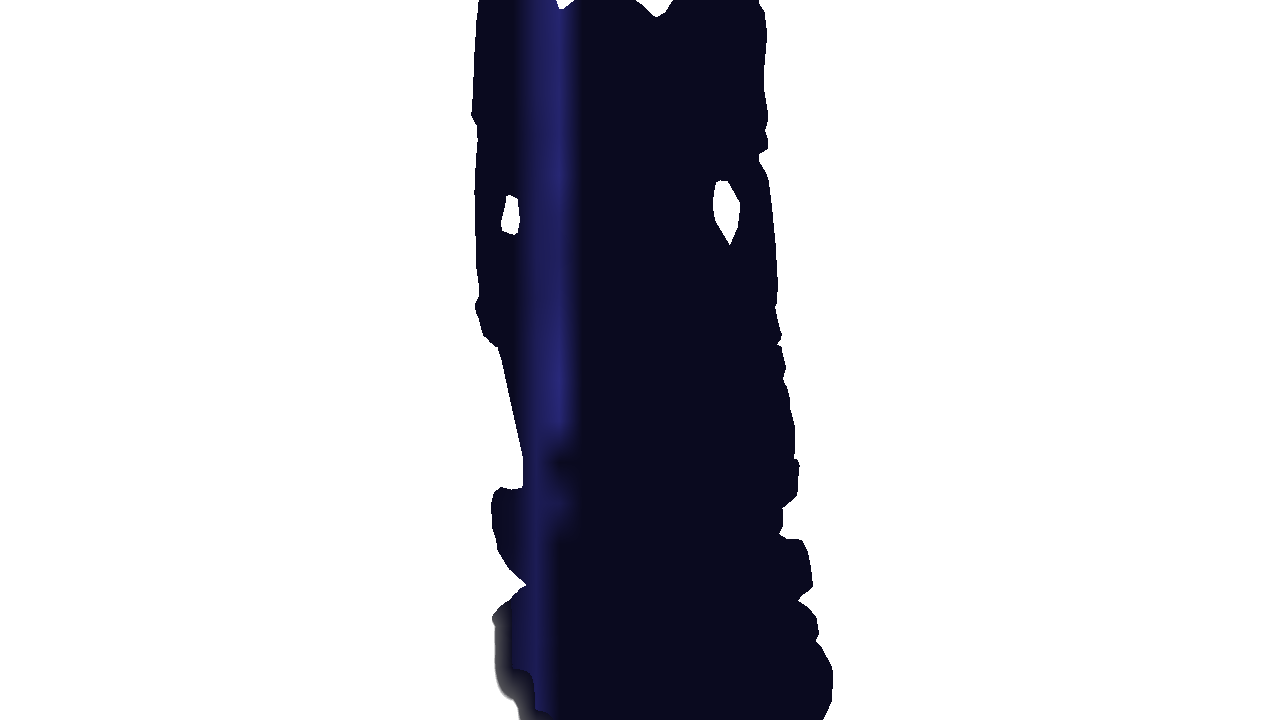
\includegraphics[scale=0.4]{images/fail_transparent.png}
\end{figure}

\section{Evaluation}
\subsection{Mémoire}
Le rendu par cette méthode peut être plus efficace en termes de consommation mémoire que le rendu du maillage détaillé. En effet, le nombre de points
de vue requis, bien que dépendant de l'objet, est relativement faible. Par exemple, le maillage du Bouddha, de l'université de Stanford, occupe 80Mo de mémoire.
En utilisant une dizaine de points de vue, et en stockant les textures à une résolution de 512$\times$512, avec un z-buffer de 16 bits, et un maillage
comptant 1\% du nombre de triangles du maillage original, la totalité des données occupe environ 20Mo.

\subsection{Temps de rendu}
L'implémentation n'étant pas fonctionelle, les chiffres sont tirés de~\cite{SG05}: une scène composée de 15 millions de triangles (15 Bouddhas) est affichée
à 2.21 images par seconde. La méthode appliquée à cette scène permet de diviser le nombre de triangles par 100 et de passer à 140 000 triangles, tout en
affichant la scène à 66.73 images par seconde. D'autres exemples montrent des améliorations de performances du même ordre de magnitude, d'un facteur allant de 20 à 30,
pour un maillage 99\% moins dense.

\subsection{Qualité des rendus}
\begin{figure}\label{fig:qualite}
    \centering
    \caption{Qualité des rendus. \`A gauche, le maillage original (1,5M triangles). \`A droite, l'application de la méthode.}
    \includegraphics[scale=0.5]{images/qualite.pdf}
\end{figure}
L'implémentation ne fonctionnant pas, le visuel est tiré de~\cite{SG05}. On constate que le rendu est d'une qualité fidèle à l'original.
On peut néanmoins remarquer 2 défauts~:
\begin{easylist}[itemize]
& Des occlusions par endroit, lorsque l'erreur commise par la méthode est trop importante, et que le pixel dessiné approxime
en fait un point différent de la surface. Ces occlusions peuvent être limitées par une augmentation de la couverture de la
surface par les points de vue. Les zones encerclées en vert sur la figure sont affectées.
& De plus, des défauts sont présents sur les bords de l'objet, où l'on distingue la géométrie du maillage simplifié. On peut
facilement l'observer dans la zone entourée en jaune.
\end{easylist}

\subsection{Conclusions}
Il ressort de l'étude que cette méthode permet un gain de performance intéressant pour les rendus de géométries suffisamment
complexes, au prix d'une légère perte de précision. La technique est de plus relativement simple et l'implémentation
s'appuie sur des fonctionnalités présentes sur virtuellement tous les matériels disponibles aujourd'hui. Cela en fait une
méthode particulièrement intéressante pour les applications où le rendu doit être fait en temps réel et où une légère perte
de qualité est acceptable.


\chapter{Améliorations}

Nous avons vu que la méthode fonctionne, mais également qu'elle présente quelques défauts. Voici mes pistes d'amélioration.
Mon implémentation n'étant pas fonctionnelle, il ne s'agit que de pistes, n'ayant pas été explorées.

\section{\'Elimination des occlusions}
Une amélioration possible serait un traitement permettant de rechercher des points/surfaces non couvertes par l'ensemble de points de vue
et souffrant du phénomène d'occlusion. Il serait ensuite possible de compléter l'ensemble par de nouveaux points de vue assurant une
meilleure visibilité de ces surfaces.

En observant le rendu des occlusions, on constate que les pixels atteints ``font t\^ache''. Cela s'explique par la nature des occlusions~:
le pixel dessiné est le résultat de la reprojection d'une mauvaise approximation du point de l'objet correspondant, ce qui explique la discontinuité observée.
Une piste prometteuse pour détecter les pixels touchés serait donc de calculer le gradient de couleur de l'image et de rechercher des discontinuités importantes.

\section{Automatisation de l'aquisition des points de vue}
Une des améliorations de la méthode sur la technique VDTM est la simplification des prétraitements. En effet, il
suffit de générer un maillage simplifié et de procéder a l'aquisition des points de vue. Cependant, cette dernière
partie requiert l'intervention de l'utilisateur. On se pose donc la question de comment automatiser ce traitement.\\
Une méthode naïve consisterait à construire un paramètrage de l'espace décrivant un ensemble de points servant de centres de projection
pour la capture des points de vue. On peut par exemple orienter la caméra vers le point de la surface le plus proche. Un exemple trivial
d'un tel paramétrage serait la sphère englobante de l'objet.\\
Cette méthode demande cependant à être affinée, car le nombre de points de vue en résultant peut devenir grand, et un critère d'orientation
peut donner de mauvais résultats.

\section{Elimination des points de vue redondants}
L'automatisation de l'aquisition risque dans tous les cas de générer un grand nombre de points de vue. Un algorithme
permettant d'éliminer de l'ensemble le point de vue apportant le moins d'information permettrait ainsi de réduire la taille
de l'ensemble tant que la suppression de points de vue ne cause pas de grosse perte de précision. Une ébauche d'un tel algorithme
peut se présenter ainsi~:

On cherche à associer à chaque point de vue de l'ensemble un coût, quantifiant la perte d'information causée par la suppression du point de vue.
La première étape est de déterminer pour chaque point de vue $V_i$ les régions de l'espace dans lesquelles placer le centre de projection de la caméra
provoquera l'utilisation de $V_i$ par la méthode. Il s'agit de l'ensemble des points $P$ tels que \[\forall{}j,k,i\neq{}j,i\neq{}k, d(P,V_i) < d(P,V_j) \text{ ou } d(P,V_i) < d(P,V_k)\]
On peut ensuite pour chacune de ces régions déterminer quel point de vue serait sélectionné à la place de $V_i$ s'il était supprimé de l'ensemble.
Il reste ensuite à faire un rendu dans les 2 cas, puis à quantifier la perte d'information d'un cas à l'autre, par rapport au rendu de référence.
Il est envisageable de répéter ce procédé tant que la perte ne dépasse pas un certain seuil.


\bibliographystyle{plain-fr}
\bibliography{rapport}
\end{document}
